% sips -s format png your_pdf_file.pdf --out your_png_file.png

\documentclass[tikz,border=0mm]{standalone}

\usepackage{amsmath}
\usepackage{graphicx}
\usepackage[T1]{fontenc}
\renewcommand\familydefault{\sfdefault} 

\usetikzlibrary{arrows,shapes,calc,math,decorations.fractals,patterns,backgrounds,decorations.markings,decorations.pathmorphing}

\tikzset{point/.style={fill,circle,inner sep=1.5pt}}
\tikzset{vector/.style={-triangle 45, line width=1pt}}
\tikzset{dblarrow/.style={latex'-latex'}}
\tikzset{partial ellipse/.style args={#1:#2:#3}{insert path={+ (#1:#3) arc (#1:#2:#3)}}}
\tikzset{xaxis/.style={-stealth',red,line width=1pt}}
\tikzset{yaxis/.style={-stealth',green!80!black,line width=1pt}}
\tikzset{zaxis/.style={-stealth',blue,line width=1pt}}
\renewcommand{\vec}{\mathbf}


\begin{document}

% Spyder window
\begin{tikzpicture}
    \node {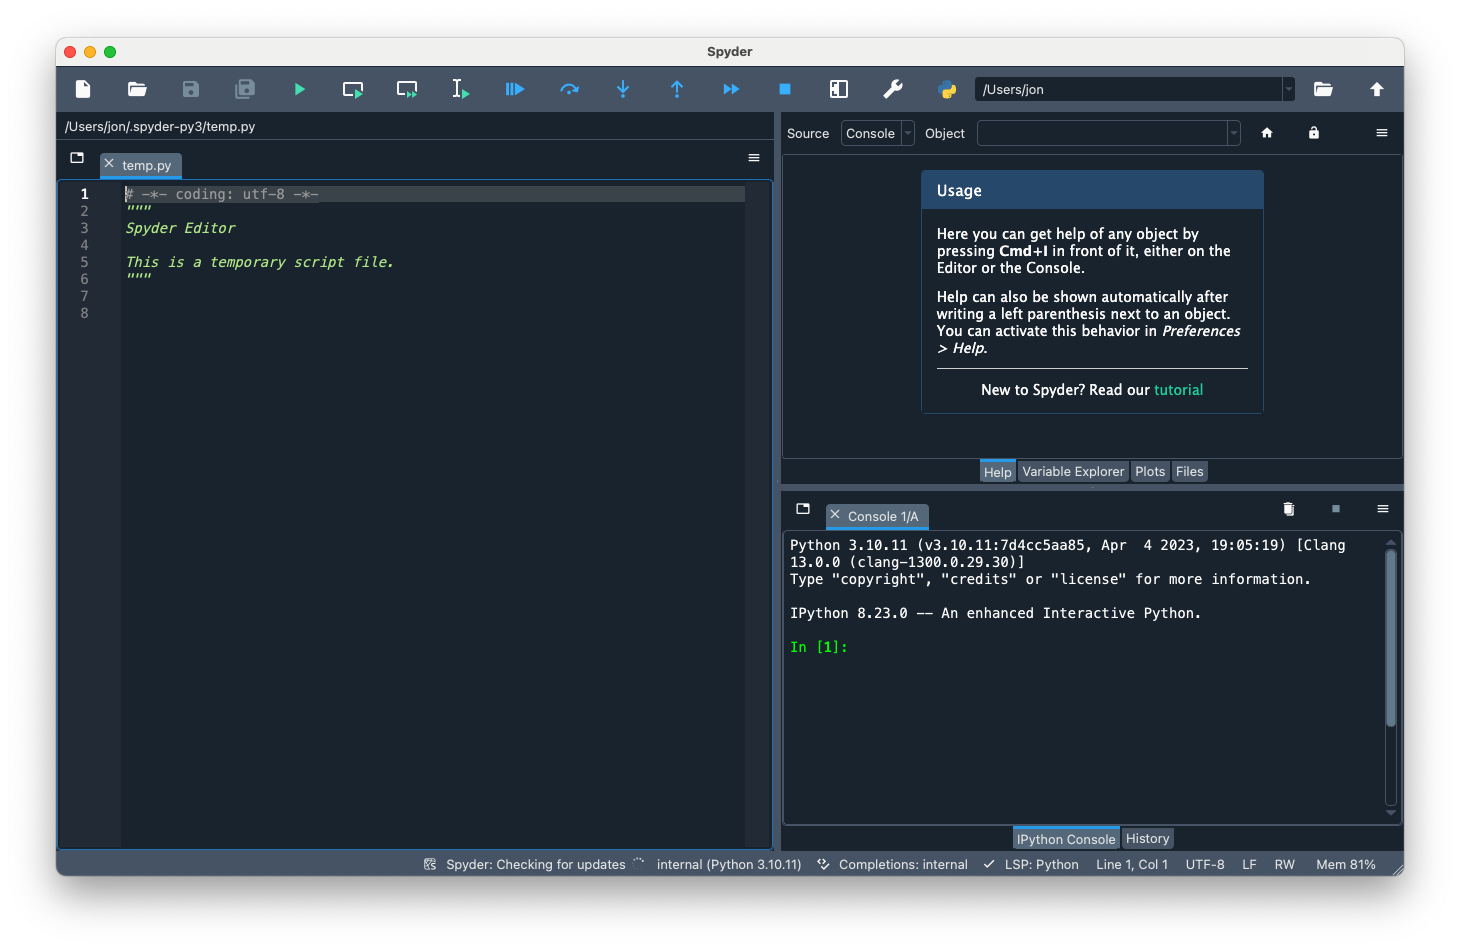
\includegraphics{../1_Spyder.png}};
    \draw [red,line width=4pt] (2,-13.2) rectangle ++(21.7,12.5);
    \node [red] at ($(2,-13.2)!0.5!(23.7,-1)$) {\Huge \bf Console window};
    \draw [green,line width=4pt] (-23.5, -13.2) rectangle ++(25,25);
    \node [green] at ($(-23.5,-13.2)!0.5!(1.5,11.8)$) {\Huge \bf Editor window};
\end{tikzpicture}

\end{document}